% This file describes the general structure of some of our sm_sir models.
% Note that it is possible to construct models in many different ways using the sm_sir code.
% Therefore, this description should be used with caution, because it only describes one possible model configuration.

\section{Model description}

\subsection{General approach}
We use a semi-mechanistic compartmental model of COVID-19 transmission governed by ordinary differential equations (ODEs). 
Our model captures important factors of COVID-19 transmission and disease such as age-specific characteristics, 
heterogeneous mixing, vaccination and the emergence of different variants of concern. 
The ODE-based model is used to capture only states relevant to transmission, whereas hospitalisations and deaths are
estimated through a convolution process. This process combines the model-estimated disease incidence with 
statistical distributions modelling the time to hospitalisation, the hospital stay duration and the time to death.
This approach presents two main advantages. First it reduces the complexity of the dynamic system relying on 
numerical solving of ODEs, which is computationally expensive. Second, the convolution approach allows for more flexibility 
and produces more realistic assumptions regarding the timings of hospitalisations and deaths, 
compared to what could be achieved with a simple compartmental approach. The following sections describe the model in details.

% ____________________________________________________
% Let's talk about the transmission model
%______________________________________________________

\subsection{Transmission model}
\label{trans} 
\subsubsection{Compartment types and sequence}
Model compartments represent sequential progressions through the processes of 
infection with, progression through, and recovery from the phases of SARS-CoV-2
infection and COVID-19 disease. The following types of compartments are implemented:
\begin{itemize}
    \item Susceptible
    \begin{itemize}
        \item Persons never previously infected with SARS-CoV-2 during or before the model simulation period
    \end{itemize}
    \item Latent
    \begin{itemize}
        \item Persons recently infected with SARS-CoV-2, but not in the active phase of the disease yet.
        \item These individuals may still be infectious (see details in next paragraph).
    \end{itemize}
    \item Active
    \begin{itemize}
        \item Persons with active COVID-19 who are currently infectious.
    \end{itemize}
    \item Recovered
    \begin{itemize}
        \item Persons recovered from COVID-19 during the model simulation period       
        \item Reinfection from these compartments is permitted through exposure to a different
        strain than the one that most recently infected the individual (see strain stratification section for details).
    \end{itemize}
\end{itemize}
The base model structure consists of a sequence of one susceptible compartment ($S$), four latent compartments ($E_1$, ..., $E_4$), four active disease compartments ($I^1$, ..., $I^4$) and one recovered compartment ($R$) (Figure \ref{fig:se4i4r}).

\begin{figure}[ht]
    \begin{center}
    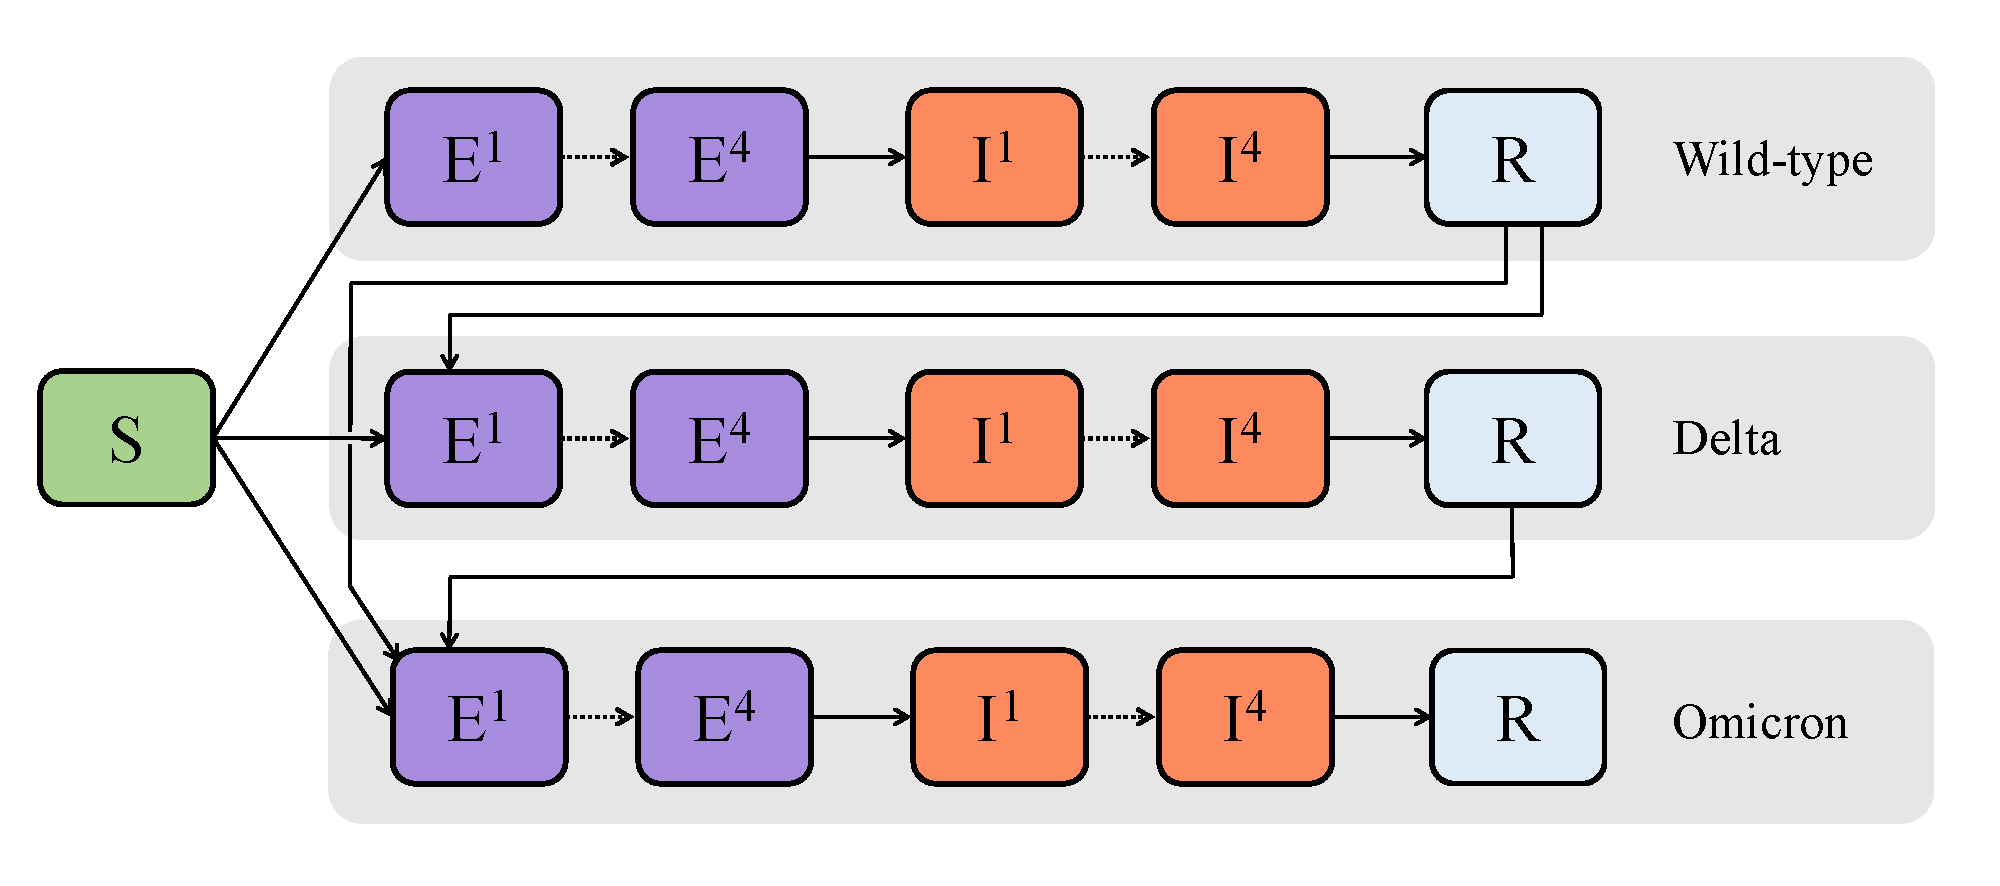
\includegraphics[width=0.75\textwidth]{../../tex_descriptions/models/sm_covid/sm_covid_se4i4r.pdf}
    \end{center}
    \caption{Compartmental model structure. 
    S = Susceptible, E = Exposed / Latent, I = Active disease, R = Recovered.
    Stratification by age and vaccination status are not shown here.
    } 
    \label{fig:se4i4r}
\end{figure}

The main rationale for using four serial compartments for both the latent and active states is to achieve an Erlang distribution for the time spent in each of these states. This distribution is more realistic than
the exponential distribution that would have been associated with a single compartment, because the Erlang distribution does not have a large density mass around 0 and is not heavy-tailed. Figure [\textcolor{red}{add Fig Ref}] 
illustrates the modelled distributions of the 
The four active disease compartments have all exactly the same characteristics. However, the last two latent compartments ($E^3$ and $E^4$) are infectious whereas the first two ($E^1$ and $E^2$) are not. We further assume that 
the infectious latent compartments are half as infectious as the active disease compartments.

\subsubsection{Model stratification by age}
\label{age}
\subsection{Model stratification}
% Note that this will vary for every application, so will need to be edited - not sure of how best to manage this:
All compartments of the base compartmental structure were stratified by age, location and organ status:\linebreak
Age
\begin{itemize}
    \item Zero to 14 years
    \item 15 to 24 years
    \item 25 to 49 years
    \item 50 to 69 years
    \item 70 years and above
\end{itemize}
Location
\begin{itemize}
    \item South Tarawa
    \item Other location
\end{itemize}
Organ status
\begin{itemize}
    \item Pulmonary smear-posivtive
    \item Pulmonary smear-negative
    \item Extrapulmonary
\end{itemize}


\subsubsection{Capturing the effects of vaccination}

History of vaccination was captured by stratifying all model compartments by vaccination status.
Two vaccination strata were included to represent those who have received at least two doses of a COVID-19 vaccine,
and those who have not.

We used data from \textit{Our World in Data} to inform the modelled dynamic vaccination coverage \cite{mathieu2021}. In particular, we specified the time-variant proportion of vaccinated people 
in our model using the reported proportion of people ``fully vaccinated'', defined as individuals who have received all doses for a prescribed vaccination protocol for a general population. We assumed that older individuals are vaccinated 
first by prioritising the modelled age groups in descending order, to align with WHO policy to prioritise the vaccination of older adults within the general population \cite{whovax2020}. That is, the oldest age group receives all available vaccines until a 
saturation coverage of 80\% is reached for this group. Then the next oldest category starts receiving vaccines and we repeat this process until all available vaccines
are allocated. Note that in the event that the population-level vaccine coverage exceeds 80\%, the saturation coverage was set equal to the population-level coverage. 

Let us consider two successive time points $t_i$ and $t_{i+1}$ for which vaccination data are available. Let us denote $r_{a, i}$ and $r_{a, i+1}$ the associated vaccine 
coverage for age group $a$. The time-variant and age-specific vaccination rate per capita $\omega_a(t)$ verifies:

\begin{equation}
    1 - r_{a, i+1} = (1 - r_{a, i})e^{-w_a(t)(t_{i+1} - t_i)} \quad, \forall t \in [t_i, t_{i+1}) .
\end{equation}

Then, 
\begin{equation}
    \label{eq:vacc}
    \omega_a(t) = \frac{\ln(1 - r_{a, i}) - \ln(1 - r_{a, i+1})}{t_{i+1} - t_i} \quad, \forall t \in [t_i, t_{i+1}) ,
\end{equation}
where $\ln(x)$ represents the natural logarithm of $x$.

Figure \ref{fig:vaccination} shows the modelled vaccination coverage over time against the reported data for the analysed countries.

\begin{figure}[h]
    \begin{center}
    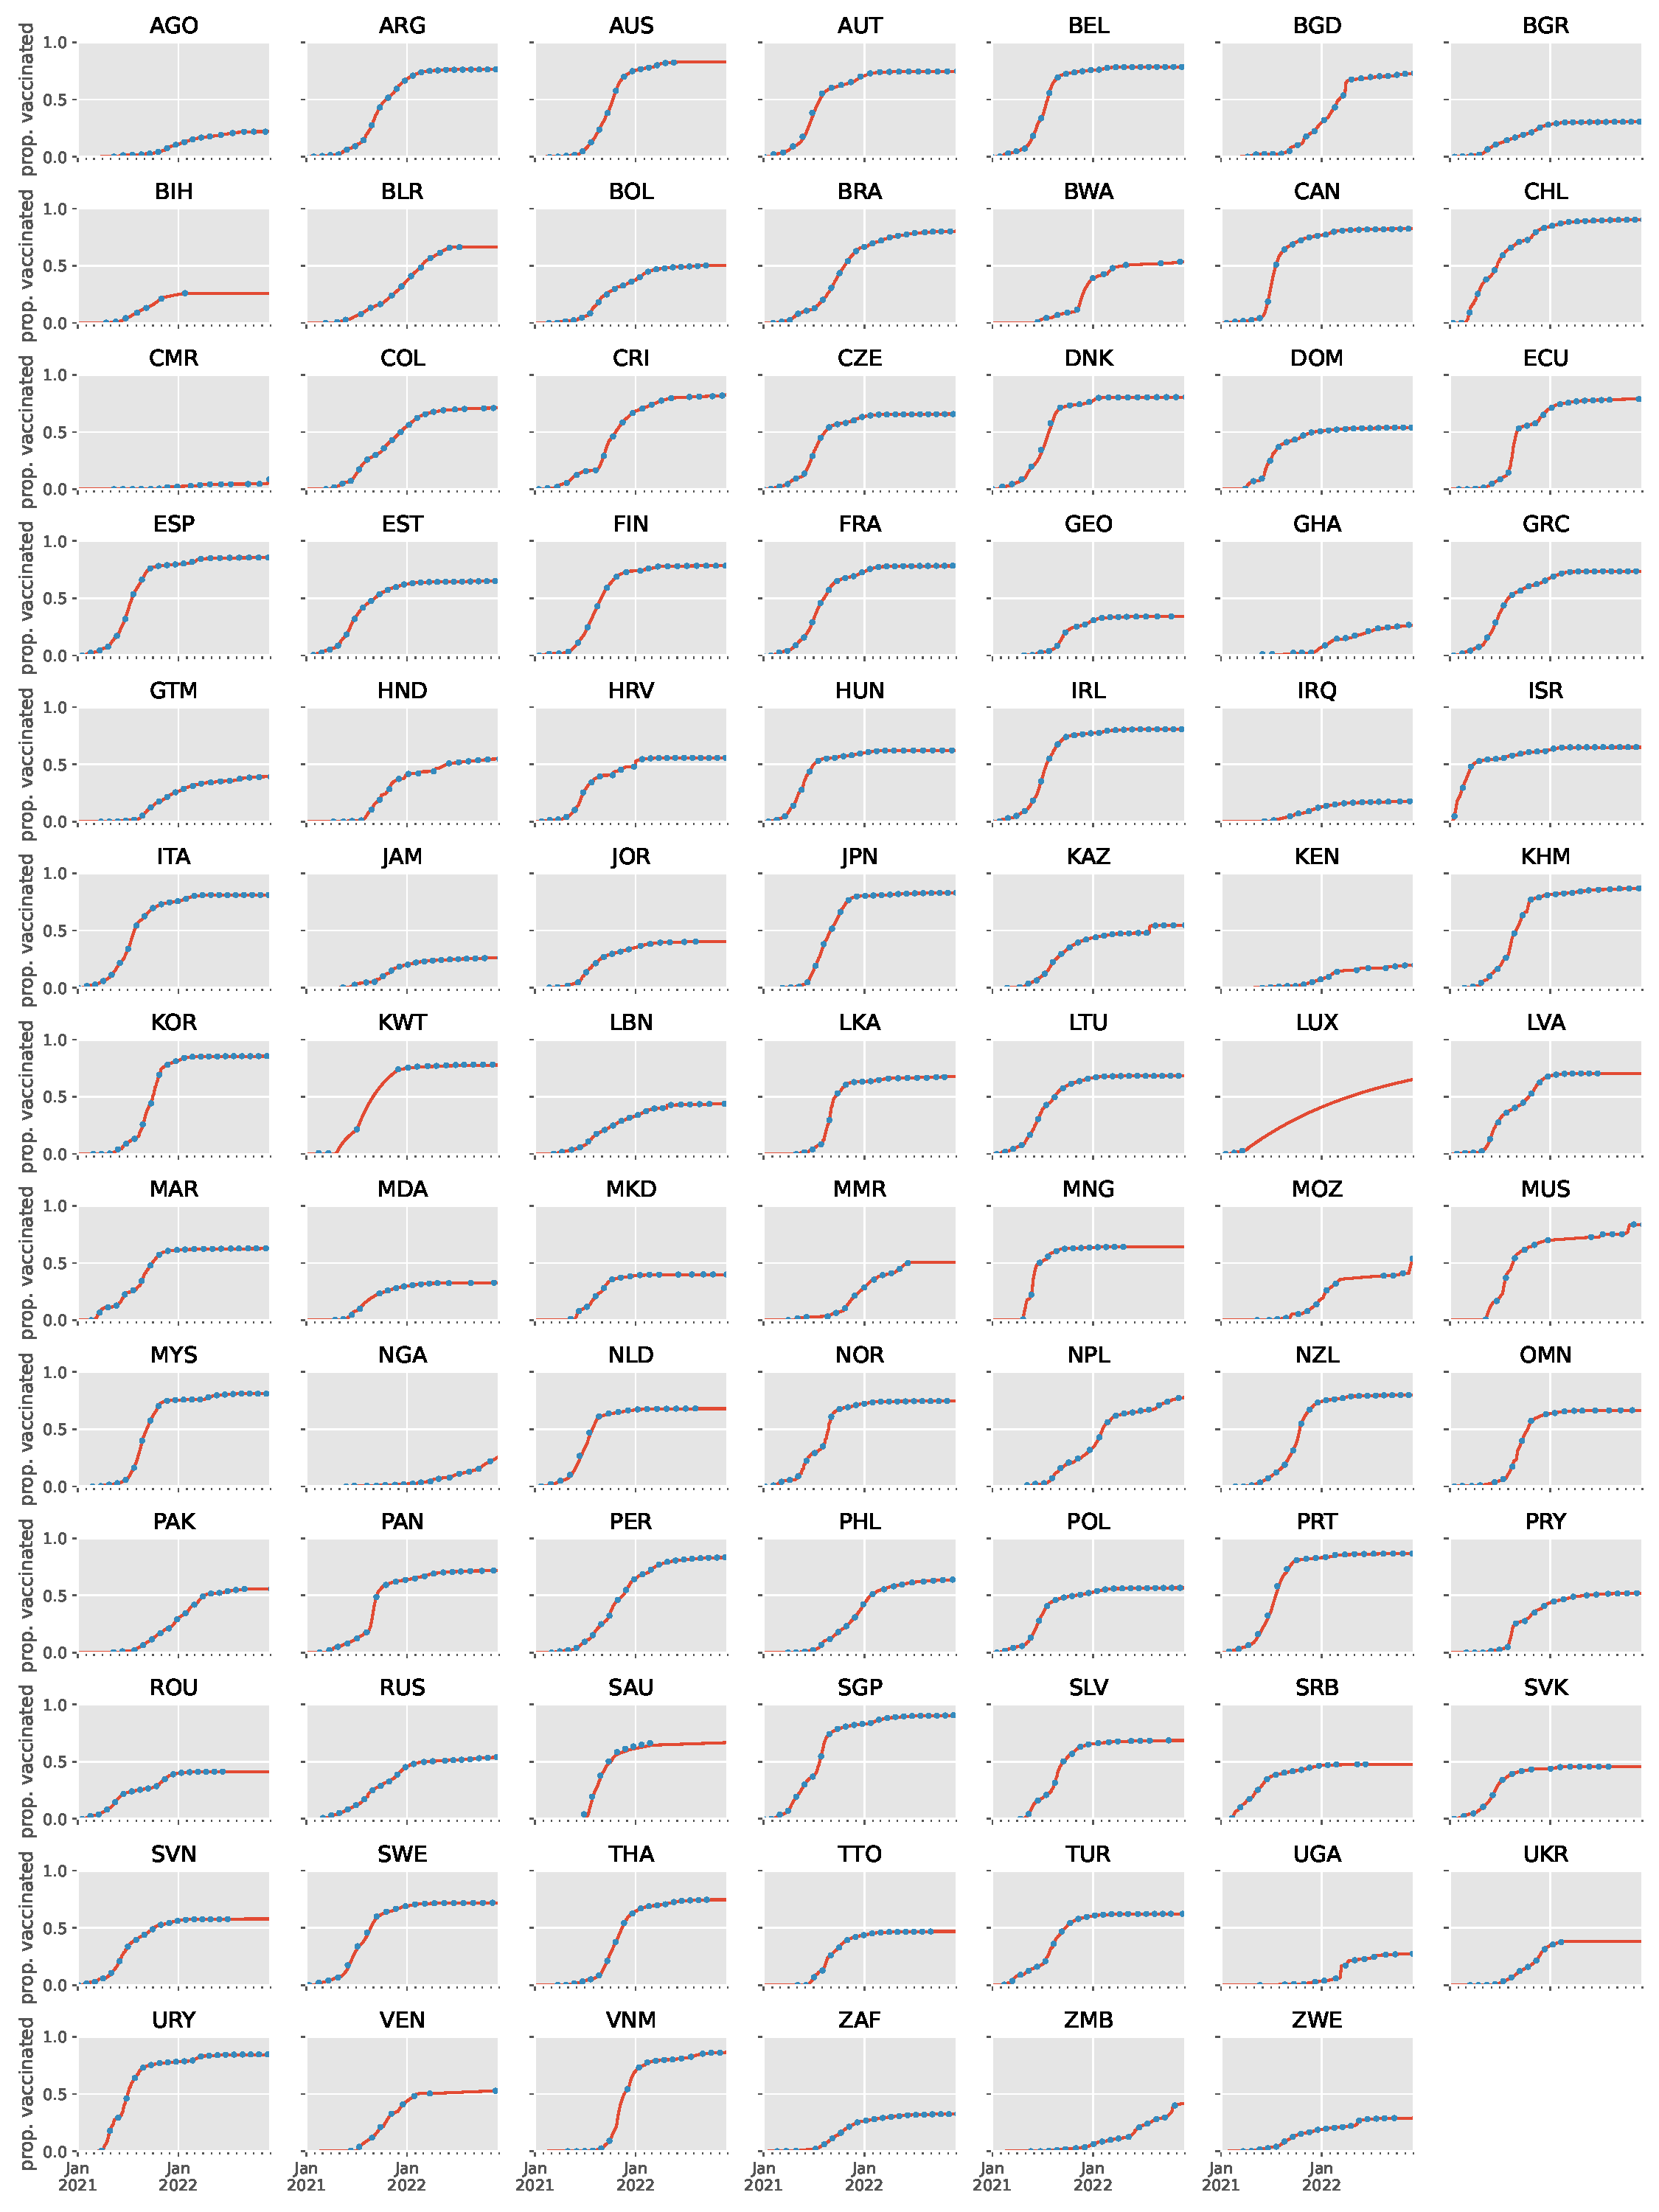
\includegraphics[width=1.0\textwidth]{../../tex_descriptions/projects/sm_covid/vacc_coverage.pdf}
    \end{center}
    \caption{Modelled vaccine coverage (lines) against data (dots).
    } 
    \label{fig:vaccination}
\end{figure}

The effect of vaccination on transmission is to reduce the rate of infection partially for all persons at risk of infection in the vaccinated stratum.
This includes both fully susceptible (never previously infected) persons,
as well as recovered persons who are at risk of reinfection. The model allows for hybrid immunity
in the sense that the vaccination-induced relative reduction of transmission risk is multiplied with that induced by previous infection. Vaccination is also assumed to reduce the risk of hospitalisation and death. 

Emerging variants of concern (VoCs) may partially escape vaccine-induced (as well as infection-induced) immunity, as described further below (Table \ref{param_table} and Section \ref{strains}).

\subsubsection{Modelling multiple viral strains}

The model was stratified by ``strain'' to simulate the emergence of multiple variants of concern (VoC).
This approach explicitly represents multiple competing strains, each with an independent force of infection calculation.
We assumed that VoCs can have different levels of transmissibility, incubation period and disease severity 
(hospitalisation and death risks) compared to the ancestral COVID-19 strain. In addition, VoCs were assumed to escape 
immunity partially for both vaccination- and infection-related immunity. 

We assumed that individuals previously infected with the wild-type strain could only be reinfected with the delta or 
omicron strains. However, such individuals have a reduced risk of infection with these variants compared to 
infection-naive individuals (82\% and 45\% reduction for delta and omicron, respectively) \cite{stein2023}.
We assumed that individuals previously infected with the delta variant could only be reinfected with the omicron variant, 
with an infection risk reduced by 45\% compared to infection-naive individuals \cite{stein2023}. 
The other parameters used to represent strain-specific characteristics are presented in Table \ref{param_table}.

Seeding of each new strain into the model was achieved through the importation of a small number (10 per million population) of new infectious persons with the relevant strain into the model.
The seeding process was implemented over a ten-day period, with the start of this period extracted from the GISAID database for each country \cite{gisaid2023}. 
We considered a strain (either Delta or Omicron) to have emerged when, during a single week in GISAID, at least two cases of that strain were reported, and these cases accounted for at least 1\% of all reported cases during that week.
 


\subsubsection{Dynamic social mixing}
Mixing matrices.

Google data.

School closure.

\subsubsection{Random transmission adjustment}
The risk of SARS-CoV2 transmission per contact is adjusted by a time-variant random process, making
the model semi-mechanistic. This random process reflects the fact that all the variations observed in the transmission
risk cannot be explained solely by the factors that are included explicitly in the model such as vaccination, dynamic mobility or new variants' emergence.
We therefore allow for random perturbations to the risk of transmission over time, although these perturbation are highly auto-correlated
to avoid significant changes in short periods of time.

We use a Wiener process $W(t)$  defined by:

\begin{equation}
    \begin{split}
    W(0) & = 0 \\
    W(t+1) & \sim \mathcal{N}(W(t), \epsilon) \quad ,
    \end{split}
\end{equation}

where $\mathcal{N}$ denotes the Normal distribution and where the standard deviation $\epsilon$ is automatically calibrated by the MCMC.
The Wiener process is updated on a fortnightly basis and is exponentiated before being applied to the risk of transmission per contact (see Equation \ref{foi}). 

\subsubsection{Ordinary differential equations}
\label{ODEs}
We now introduce some new notation. Modelled age groups are indicated by the subscript $a$, and $\mathcal{A}$ represents
the set of all modelled age groups (see Section \ref{age}). Vaccination status is represented by the subscript $v$, and $\mathcal{V}$ is the set of 
vaccination statuses (i.e. $\mathcal{V}=$ \{``0'', ``1''\}, where ``0'' represents unvaccinated people and ``1'' represents vaccinated people). The subscript $s$ is used to represent the different viral strains, and $\mathcal{S}$ is the set 
of all strains (i.e. $\mathcal{S}=$ \{``wild-type'', ``delta'', ``omicron''\}). The average incubation period duration associated with strain $s$ is denoted $q_s$ and
the average duration of active disease is denoted $w$. The relative susceptibility to infection with strain $s$ of individuals aged $a$ with 
vaccination status $v$ is denoted $\rho_{a,v,s}$. The term $b_{a,v,s}(t)$ designates the introduction of individuals of age $a$ and 
with vaccination status $v$ that are infected with strain $s$ (infection seeding). Vaccination is characterised by the age-specific
and time-variant per-capita vaccination rate $\omega_a$. Finally, $\chi_{s,\sigma}$ represents the relative susceptibility to infection
with strain $\sigma$ for individuals whose most recent infection episode was with strain $s$. Using this new notation combined 
with those previously introduced, we can describe the transmission model with the following set of ordinary differential equations:

\begin{equation}
    \label{ode}
    \begin{split}
\frac{dS_{a,v}}{dt} & = -\sum_{s \in \mathcal{S}} \lambda_{a,s}(t)\rho_{a,v,s} S_{a,v} + \Phi_v\omega_a(t)S_{a,v=0}  \quad , \\
\frac{dE_{a,v,s}^{1}}{dt} & =\lambda_{a,s}(t)\rho_{a,v,s} \Bigl(S_{a,v}  +  \sum_{\sigma \in \mathcal{S}} \chi_{\sigma, s} R_{a,v,\sigma} \Bigr) - \frac{4}{q_{s}}E_{a,v,s}^{1} + \Phi_v\omega_a(t)E_{a,v=0,s}^1 \quad , \\
\frac{dE_{a,v,s}^{k}}{dt} & = \frac{4}{q_{s}}E_{a,v,s}^{k-1} - \frac{4}{q_{s}}E_{a,v,s}^{k} + \Phi_v\omega_a(t)E_{a,v=0,s}^k \quad,  \forall k \in \{2,3,4\} , \\
\frac{dI_{a,v,s}^{1}}{dt} & = \frac{4}{q_{s}}E_{a,v,s}^{4} - \frac{4}{w}I_{a,v,s}^{1} + b_{a,v,s}(t) + \Phi_v\omega_a(t)I_{a,v=0,s}^1 \quad , \\
\frac{dI_{a,v,s}^{k}}{dt} & = \frac{4}{w}I_{a,v,s}^{k-1} - \frac{4}{w}I_{a,v,s}^{k} + \Phi_v\omega_a(t)I_{a,v=0,s}^k \quad, \forall k \in \{2,3,4\} , \\
\frac{dR_{a,v,s}}{dt} & = \frac{4}{w}I_{a,v,s}^{4} - \sum _{\sigma \in \mathcal{S}} \lambda_{a,\sigma}(t)\rho_{a,v,\sigma} \chi_{s, \sigma} R_{a,v, s} + \Phi_v\omega_a(t)R_{a,v=0,s} \quad, 
    \end{split}
\end{equation}

where $\lambda_{a,s}$ represents the force of infection of strain $s$ affecting individuals of age $a$. The quantity $\Phi_v$ is a binary variable
used to switch between a positive and negative multiplier depending on vaccination status. It is equal to $1$ when
$v=$``1'' and $-1$ when $v=$``0''. In other words, $\Phi_v = 2\mathbbm{1}_{v=``1"} - 1$. 

The force of infection was calculated as:
\begin{equation}
    \label{foi}
 \lambda_{a,s}(t) = \beta e^{2W(t)} \psi_{s} \sum_{\alpha \in \mathcal{A}} \sum_{v \in \mathcal{V}} \frac{c_{a,\alpha}(t)}{N_{\alpha, v}} \Bigl( 0.5 \sum_{k=3}^{4} E_{\alpha,v,s}^{k} + \sum_{k=1}^{4} I_{\alpha,v,s}^{k} \Bigr) \quad .
\end{equation}
In the previous equation, $\beta$ represents the unadjusted risk of transmission per contact, $\psi_{s}$ is the relative infectiousness of strain $s$, and $W(t)$ is
the random process introduced in Section \ref{random_process}. The size of the population of age $\alpha$ with vaccination status $v$ is denoted $N_{\alpha, v}$. The term $c_{a,\alpha}(t)$ is a single element of the contact matrix $C(t)$ introduced in Equation \ref{eq_mixing}. It
represents the average numbers of contacts per day that a individual of age $a$ has with individuals of age $\alpha$. 



% ____________________________________________________
% Now, let's talk about the convolution processes
%______________________________________________________
\subsection{Estimation of COVID-19-related hospital pressure and deaths}
The transmission model described in Section \ref{trans} provides estimates of COVID-19 incidence over time, disaggregated by age, vaccination status and strain. 
We combine these incidence estimates with the age-, vaccination- and strain-specific risks of hospitalisation and deaths as well as 
statistical distributions of time to events to compute COVID-19-related hospital pressure and deaths over time.

\subsubsection{COVID-19-related hospital pressure}
\label{hosp}
The risk of hospitalisation given infection is expected to vary dramatically by setting.
For example, different countries may have different criteria for whether or not a COVID-19 
patient should be admitted to a hospital. This makes it difficult to provide accurate 
estimates of hospitalisation rates for multiple countries. 

This is why we introduce a universal indicator named ``hospital pressure'' in our analysis. This indicator
is obtained by considering the age-specific risk of hospitalisation given infection observed in the first year
of the pandemic in the Netherlands, adjusted for vaccination status and for the infecting strain (\textcolor{red}{See Table XX}).
The ``hospital pressure'' indicator can therefore be interpreted as the level of hospital occupancy that
would be observed in the analysed country if the rates of hospitalisation given infection in this country were the same
as in the Netherlands. This indicator is expected to be approximately proportional to the actual hospital occupancy level of the 
studied country. Note that this indicator is used in order to make comparisons between scenarios such that one should interpret the relative
differences between scenarios rather than the absolute values of the indicator. 

Let us denote $i_{a,v,s}(t)$ the number of new disease episodes estimated to start at time $t$ for people aged $a$ with vaccination status $v$
and infected with strain $s$. The number of new hospital admissions occurring at time $t$ is calculated using the following
convolution product:
\begin{equation}
 \eta(t) = \sum_{a,v,s} \kappa_{a,v,s} \int_{u \geq 0}  i_{a,v,s}(t-u)g_{h}(u) du   \quad,
 \end{equation}
where $\kappa_{a,v,s}$ is the risk of hospitalisation given infection for age $a$, vaccination status $v$ and strain $s$ 
based on the Netherlands data, and $g_h$ is the probability density function of the statistical distribution chosen to represent the 
time from symptom onset to hospitalisation (\textcolor{red}{See Table XX}). 

We then compute the ``hospital pressure'' quantity $h$, which is an indicator of hospital occupancy level, by combining the number of new 
hospital admissions $\eta$ with the statistical distribution used to model hospital stay duration:
\begin{equation}
h(t) = \int_{u \geq 0}  \eta(t-u) (1 - \tau(u)) du   \quad,
\end{equation}
where $\tau$ is the cumulative density function of the statistical distribution chosen to represent the 
hospital stay duration (\textcolor{red}{See Table XX}). 
 

\subsubsection{COVID-19 deaths}
We estimate the number of COVID-19 deaths over time using a similar approach 
as for the hospital pressure indicator. We use the age-specific infection fatality rates reported in
ODriscoll et al. \cite{odriscoll-2021}, adjusted for vaccination status and for the infecting strain
to estimate COVID-19 mortality. Using the same notations as in Section \ref{hosp}, the number of COVID-19
deaths observed at time $t$ is obtained by:
\begin{equation}
\mu(t) = m_C \sum_{a,v,s} ifr_{a,v,s} \int_{u \geq 0}  i_{a,v,s}(t-u)g_{d}(u) du   \quad,
\end{equation}
where $ifr_{a,v,s}$ is the risk of death given infection for age $a$, vaccination status $v$ and strain $s$, 
and $g_d$ is the probability density function of the statistical distribution chosen to represent the 
time from symptom onset to death (\textcolor{red}{See Table XX}). We use a country-specific adjuster $m_C$ to 
capture the fact that the infection fatality ratio is expected to vary by country, in part due to 
differences in COVID-19 death definition and reporting standards. This adjustment is automatically calibrated 
by the MCMC (Section \ref{calibration}). 

